
\newpage
% Rimuove intestazioni, piè di pagina e numerazione della pagina
\thispagestyle{empty}

% Riempe lo spazio superiore, spingendo il contenuto verso il basso
%\vspace*{\fill}




\begin{flushright}
	I dedicate this thesis to my wife Mariangela,\\ who has always supported me through these years,\\ to my daughter Beatrice, who gave me the strength to keep going,\\ and to my friend Enea, who has made my days brighter.
\end{flushright}
\vspace*{\fill}
\begin{comment}
	\begin{figure}[!b]
		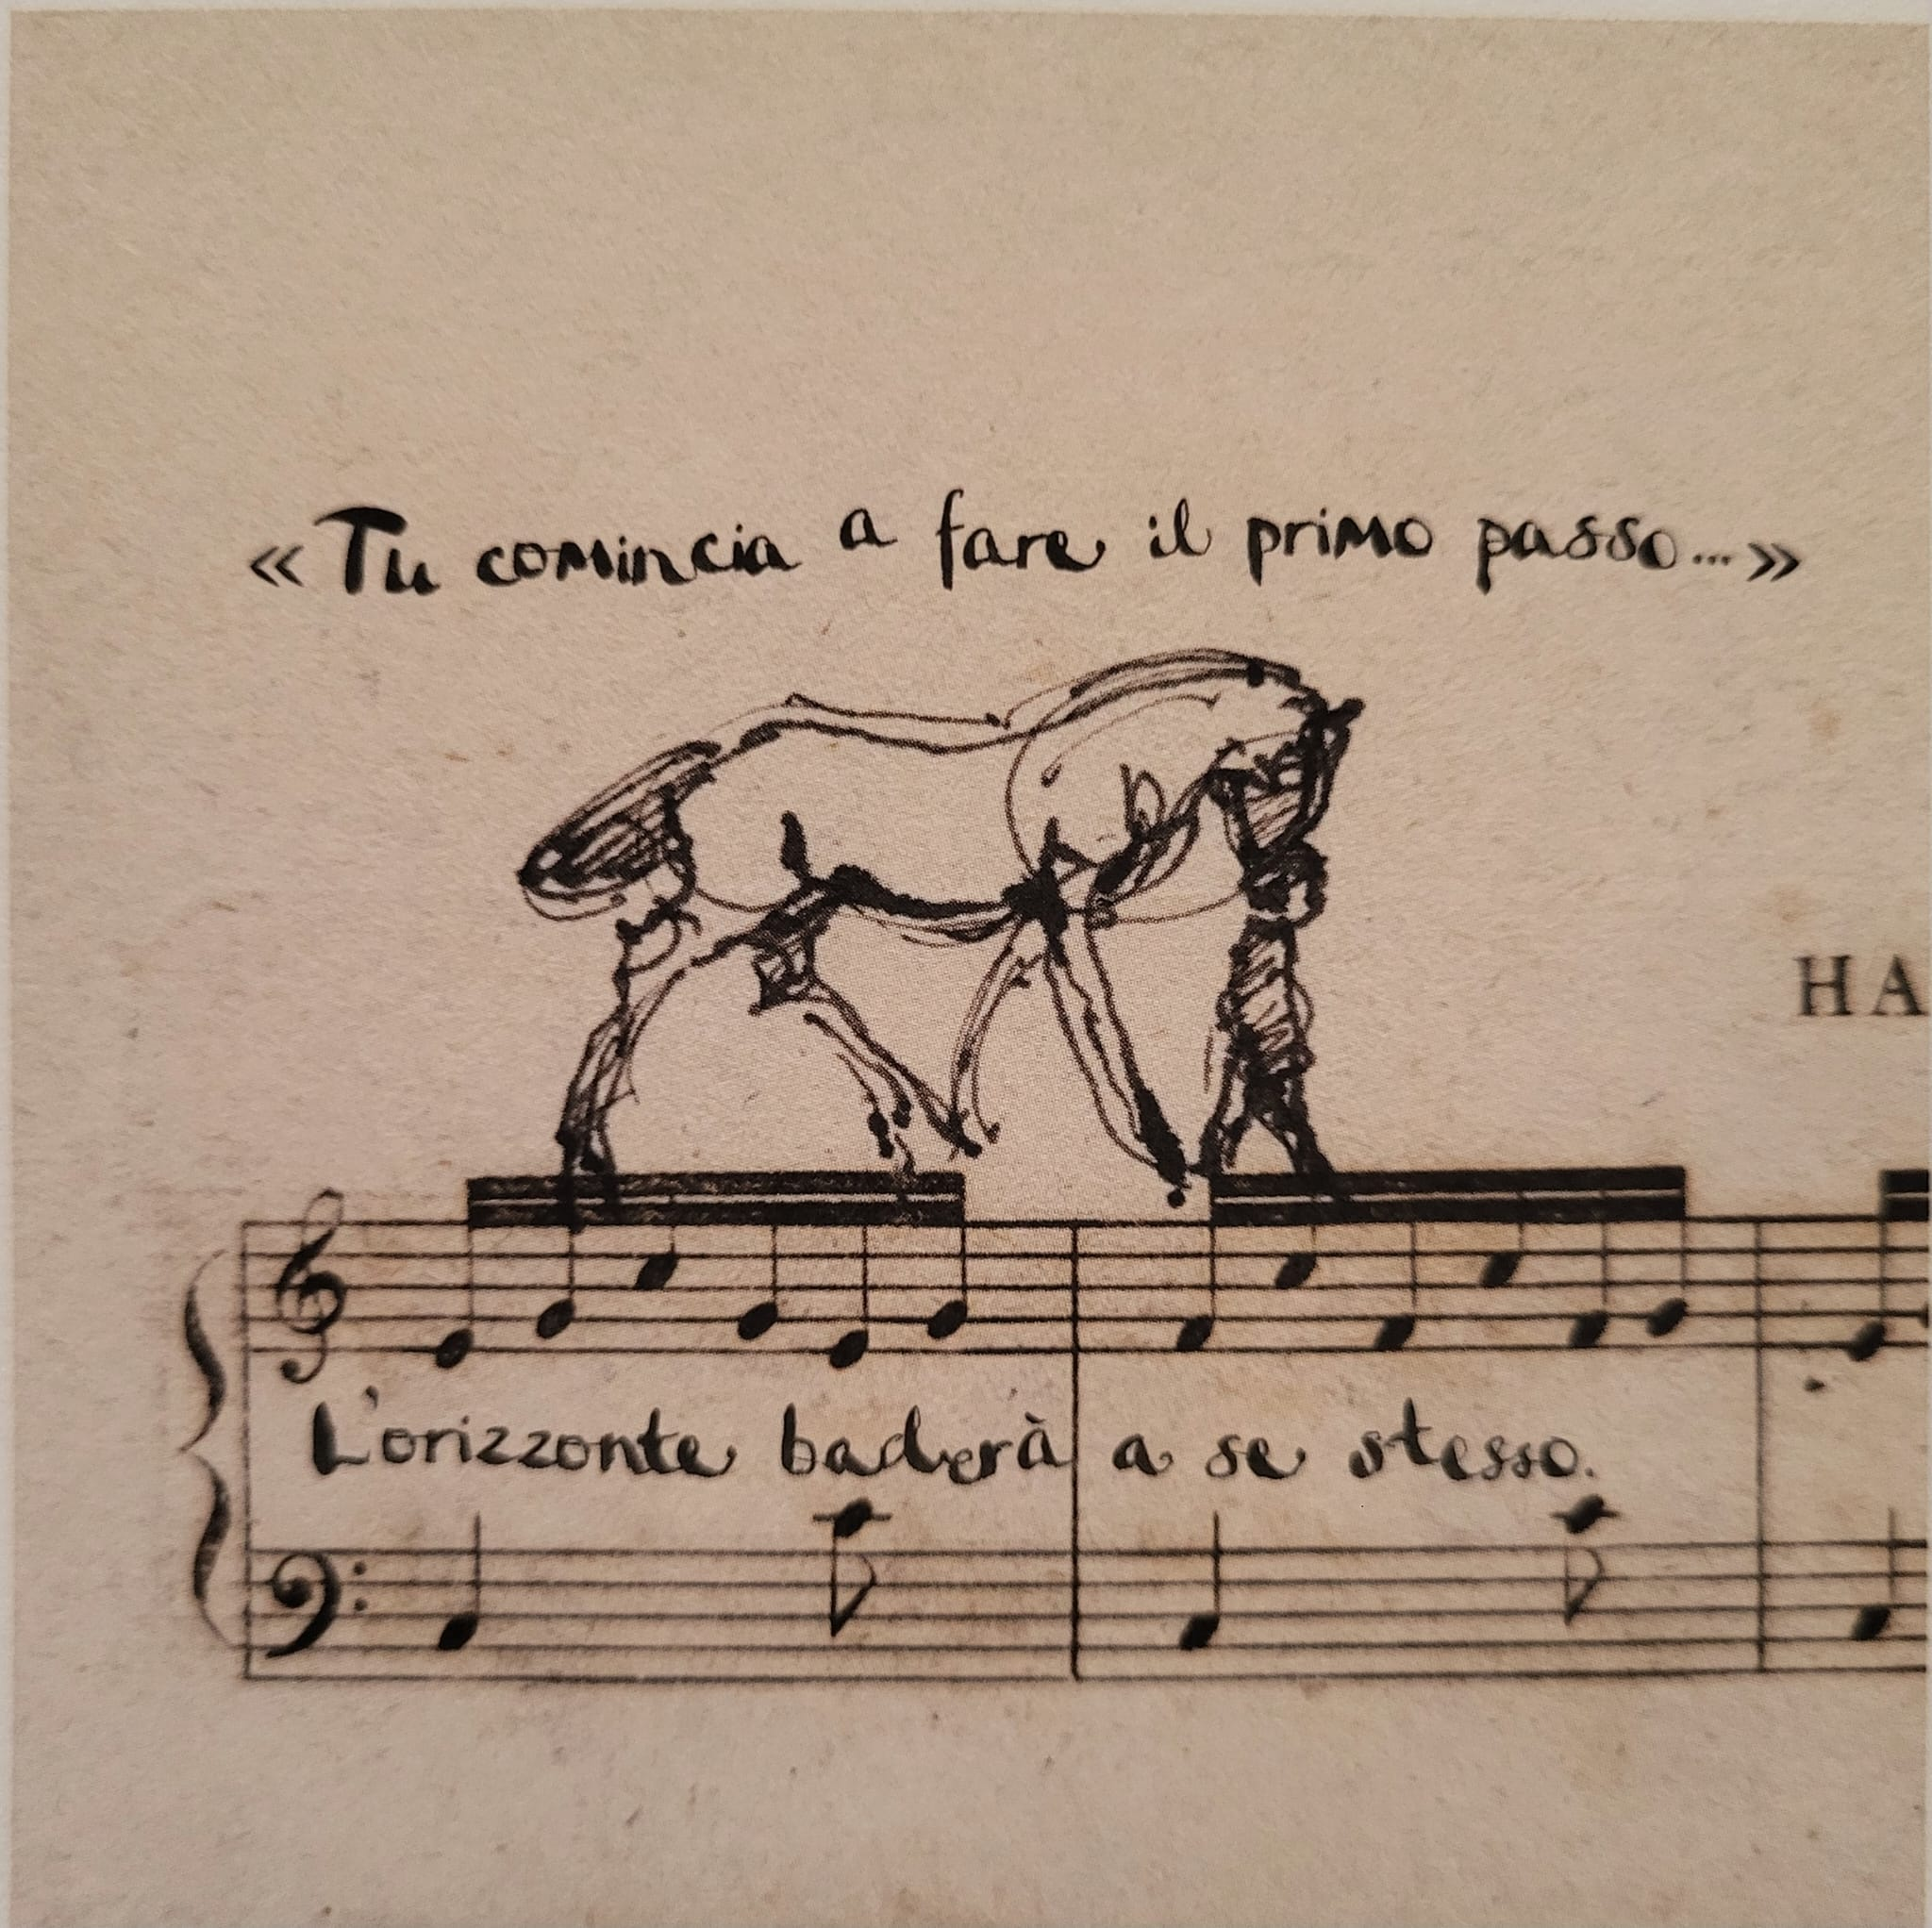
\includegraphics[scale=0.1]{figure/cavallo.jpg}
		\label{fig:dedica}
	\end{figure}
\end{comment}


\newpage
% Rimuove intestazioni, piè di pagina e numerazione della pagina
\thispagestyle{empty}











\chapter*{Abstract}
\addcontentsline{toc}{chapter}{Abstract}

This thesis investigates critical advancements in perception, learning, and cooperation mechanisms for autonomous vehicles, addressing key challenges in their development and deployment. It explores how autonomous vehicles can better perceive their environment, learn from dynamic conditions, and cooperate effectively to enhance performance, safety, and reliability.

To tackle these challenges, a comprehensive approach combining theoretical analysis, algorithm development, and practical validation was employed. The research developed an enhanced vision-based path following algorithm for UAVs, a real-time lane detection method, and a reinforcement learning strategy for pedestrian collision avoidance. Additionally, a cybersecurity framework was introduced to detect and mitigate cyber-attacks in real-time, and a robust control system was designed to enhance cooperation between autonomous vehicles in complex environments.

These advancements contribute to the broader goal of integrating autonomous vehicles into everyday life, paving the way for safer, more efficient, and resilient autonomous vehicle systems. This research underscores the potential of combining perception, learning, and cooperation mechanisms to drive the future of autonomous vehicles.
\chapter*{Acknowledgments}




I would like to thank everyone who has been involved either directly or indirectly in
this Ph.D journey. I would like to express my deepest appreciation to all those who provided me the possibility to complete this thesis. A special gratitude I give to my supervisor, Dr. Luigi Glielmo, whose contribution in stimulating suggestions and encouragement, helped me to coordinate my research. 

Furthermore, I would also like to acknowledge with much appreciation the crucial role of the staff of Department od Engineering, who provided invaluable guidance and direction for my studies and research. Their expertise and insights were pivotal in shaping the trajectory of my academic journey, offering both support and challenge when needed to refine my work and focus. The environment they fostered not only facilitated my research but also significantly contributed to my personal and professional growth. I am deeply grateful for their mentorship and the opportunities they have provided me

I would like to extend my deepest gratitude to Davide Liuzza, Valerio Mariani, and Massimo Tipaldi for their invaluable collaboration in the writing of the contributions presented within this work. Their expertise not only enriched this research with profound scientific insights but also provided me with the encouragement and human support necessary to overcome the challenges encountered along the journey. Their dedication and commitment to excellence have been a constant source of inspiration and have significantly contributed to my personal and professional growth.

I am grateful for the beautiful moments spent throughout my Ph.D journey with colleagues Luigi, Enrico, Kishan, and Amit. Because of them, the journey was filled with friendship; thanks to our diversity of cultures, we have enriched each other. All the walks spent talking about our lives, our dreams, and the experiences we had outside the university were varied and very beautiful, and I will carry them in my heart forever.

I extend my deepest gratitude to my family, who have been my cornerstone and guiding light throughout this journey. They have instilled in me the invaluable virtues of sacrifice and resilience, teaching me to face life's challenges with grace and without a word of complaint. Through their, I have learned the profound beauty of freedom-the freedom to choose my own path, to carve out my destiny, and to live a life that is authentically mine. 

Finally, I extend my heartfelt thanks to all the friends who have stood by my side, who have given me strength, and spurred me on to pursue this goal amidst all difficulties, whether they expressed their support directly or indirectly. Their presence, encouragement, and unwavering faith in me have been sources of immense comfort and motivation, pushing me to strive further even when the path seemed insurmountable. 





\addcontentsline{toc}{chapter}{Acknowledgments}
%\lhead{\bfseries ACKNOWLEDGMENTS}